\documentclass[10pt, twocolumn]{article}

\usepackage[margin=0.75in]{geometry}
\usepackage{amsmath,amsthm,amssymb}
\usepackage{xcolor}
\usepackage{cancel}
\usepackage{graphicx}
\usepackage{changepage}
\usepackage{circuitikz}
\usepackage{pgfplots}
\usepackage{siunitx}
\usepackage{hyperref}
\usepackage{cite}
\usepackage{multicol, multirow, booktabs}
\usepackage[breakable]{tcolorbox}
\usepackage[inline]{enumitem}

\theoremstyle{definition}
\newtheorem{problem}{Problem}
\newtheorem{soln}{Solution}

\pgfplotsset{compat=newest}
\usetikzlibrary{lindenmayersystems}
\usetikzlibrary{arrows}
\usetikzlibrary{calc}

\definecolor{incolor}{HTML}{303F9F}
\definecolor{outcolor}{HTML}{D84315}
\definecolor{cellborder}{HTML}{CFCFCF}
\definecolor{cellbackground}{HTML}{F7F7F7}
\newcommand{\eq}{=}
\usetikzlibrary{positioning, fit, calc}
\pgfdeclarelayer{background}  
\pgfsetlayers{background,main}
\DeclareSIUnit[number-unit-product = {\,}]\calorie{cal}
\DeclareSIUnit[number-unit-product = {\,}]\atmosphere{atm}

\makeatletter
\newcommand{\boxspacing}{\kern\kvtcb@left@rule\kern\kvtcb@boxsep}
\makeatother
\newcommand{\prompt}[4]{
    \ttfamily\llap{{\color{#2}[#3]:\hspace{3pt}#4}}\vspace{-\baselineskip}
}

\newcommand{\thevenin}[2]{
  \begin{center}
    \begin{circuitikz} \draw
      (0,0) -- (2,0) to[battery1, l_=$V_{Th}\eq#1$] (2,2) 
      to[resistor, l_=$R_{Th}\eq#2$] (0,2)
      ;
      \draw [o-] (-.07,2.079);
      \draw [o-] (-.07,0.079);
    \end{circuitikz}
  \end{center}
}

\newcommand{\norton}[2]{
  \begin{center}
    \begin{circuitikz} \draw
      (0,0) -- (3,0) to[american current source, l_=$I_{N}\eq#1$] (3,2) -- (0,2) (2,0)
      to[resistor, l=$R_{N}\eq#2$] (2,2)
      ;
      \draw [o-] (-.07,2.079);
      \draw [o-] (-.07,0.079);
    \end{circuitikz}
  \end{center}
}

\newcommand{\highlight}[1]{\colorbox{yellow}{$\displaystyle #1$}}

\newcommand{\ti}[1]{\widetilde{#1}}

\title{Physics 2700H: Lab II}
\author{Jeremy Favro (0805980),
Manan Ravat (0791811),
Layla Scrimgeour-Brown (0766619)
 \\\emph{Department of Physics \& Astronomy}\\ Trent University, Peterborough, ON, Canada}
\date{\today}
\begin{document}
\maketitle
\begin{abstract}
  Wavelengths of emitted photons associated with electron transitions in a hydrogen atom following the Balmer series were determined utilizing both geometric and wave optics.
  Some results agreed within uncertainty with accepted values for these wavelengths. Minimal relative difference was noted between calculated and accepted values. Further
  investigation into the precision of the wave and geometric optical methods is warranted.
\end{abstract}
\section{Introduction}
In 1913 Niels Bohr created the Bohr model of the hydrogen atom. This model predicts that electron orbiting an atom exist only in discreet
energy levels. The Bohr model of the atom provided a theoretical justification for the experimentally determined Rydberg equation
which modeled the wavelength of emitted photons due to electron energy level transitions in a hydrogen atom.

In this experiment we seek to determine the wavelengths associated with electron energy level transitions between $n\geq 3$ and $n=2$.
These transitions are formally known as the H-Balmer series for a hydrogen atom and are significant as the transitions from $n\leq 5$ to $n=2$ are
easily visible to the human eye\cite{lab-manual}.

Using a hydrogen lamp a spectrally pure emission of photons of distinct wavelengths was created. Both
geometrical and wave optics were employed to observe the emission spectrum of the hydrogen lamp and calculate the associated wavelengths.
\section{Theory}
\subsection{Rydberg Equation}
First stated in 1888 by Johannes Rydberg, the Rydberg equation for hydrogen relates the vacuum wavelength, $\lambda_0$, of emitted photons due to electron energy level transitions
and the initial, $n_i$, and final, $n_f$, energy levels through which the electron passes.
\begin{equation}
  \lambda_{0}=\frac{1}{R}\left(\frac{1}{n_f^2}-\frac{1}{n_i^2}\right)^{-1}
\end{equation}
where $R$ is the Rydberg constant \cite{codata}
\subsection{Quantized Angles of Minimum Deviation}
\subsubsection{Geometrical Optics}
Employing an equilateral glass prism enables the obervation of individual wavelengths of light as each wavelength is dispersed at a different angle.
See figure \ref{pris}.
For the study of the H-Balmer spectrum specifically a prism is utilized to determine $D_m$, the smallest
angle achieved by varying the angle of incident light, known as the angle of minimum dispersion,
which can be related to the refractive index of a prism through
\begin{equation}
  n=\sin\left(\frac{A+D_m}{2}\right)/\sin\left(\frac{A}{2}\right)
\end{equation}
Which, for a prism with known Cauchy constants, $\alpha$ and $\beta$, can be combined with Cauchy's dispersion relation
\begin{equation}\label{cauchy}
  n=\alpha+\frac{\beta}{\lambda_{disp}^2}
\end{equation}
to determine the wavelength of light for a given $D_m$
\begin{equation}
  \lambda_{disp}=\sqrt{\left[\sin\left(\frac{A+D_m}{2}\right)/\sin\left(\frac{A}{2}\right)-\alpha\right]^{-1}\beta}
\end{equation}
Where $A$ is the apex angle of the prism.
\subsubsection{Ray Optics}
Utilizing a diffraction grating enables the study of individual wavelengths of light due to interference in the transmitted (or reflected) light
created by the difference in optical path between refractions. See figure \ref{grat}. For a given wavelength $\lambda_{diff}$ the locations of constructive interference can be
determined using
\begin{equation}
  m\lambda_{diff}=d\sin\theta
\end{equation}
Where $m$ is the order of the diffracted band line, $d$ is the spacing between lines on the diffraction grating, and $\theta$ the angle
of the diffracted beam relative to the incident light.
\section{Methods}
\subsection{Geometrical Optics}
Light from a hydrogen lamp is incident on an equilateral dense flint glass prism with Cauchy constants (See equation \eqref{cauchy})
$\alpha=1.5935\pm0.8\%$\cite{lab-manual}, $\beta=\qty{0.0093}{\micro\meter\squared}\pm5\%$\cite{lab-manual} and apex angle $A=\frac{180}{3}\unit{\degree}$. The viewing telescope, shown in figure \ref{app}, is positioned to the first ($\lambda_{theo}=\qty{656.28}{\nano\meter}$)
spectral line. The table on which the prism sits, or the prism itself, is then rotated until the first spectral line reaches a reversal point at which its movement changes direction.
At this reversal point, the crosshairs are aligned with the right side of the spectral line. This position is recorded using the Vernier scale. This process is repeated for the other two spectral lines,
ensuring that the prism is rotated to the angle of minimum deviation for each. See figure \ref{pris} for an illustration of a successfully constructed apparatus.
\subsection{Wave Optics}
Light from a hydrogen lamp is incident on a diffraction grating with $k=\qty{1.5d4}{lines\per inch}$. Ideally the angle of incidence is $\qty{90}{\degree}$,
however a method, which was not used in this experiment, to minimize error as a result of non-ideal alignment is discussed in section \ref{wave-err}.
The viewing telescope is positioned to the first ($\lambda_{theo}=\qty{434.05}{\nano\meter}$) spectral line and the crosshairs are aligned with the right side of
that spectral line. This position is recorded using the Vernier scale. This process is repeated for the other two spectral lines. See figure \ref{grat} for an illustration of a successfully constructed apparatus.
\vfill\eject
\section{Discussion}
Utilizing the above methods both the prism and diffraction grating produced clear and distinct spectral lines.
\subsection{Geometrical Optics}
\begin{table}[ht!]
  \centering%
  \caption{Collected angles of minimum dispersion for an H-Lamp spectrum through a dense flint glass prism and their associated calculated wavelengths.
    Measurement apparatus re-zeroed between batches. $\delta D_m$ taken to be $\qty{5}{\arcminute}$ per label on apparatus.\\}
  \begin{tabular}{lllll}
    \toprule
    Colour & $\lambda_{theo}\, (\unit{\nano\meter})$ & $D_m\, (\unit{\degree})$        & $\lambda_{disp}\, (\unit{\nano\meter})$ & \% Diff \\
    \midrule
    Red    & 656.28                                  & $47.75 \pm \qty{5}{\arcminute}$ & $650.70 \pm 5$                          & 0.85    \\
    Teal   & 486.14                                  & $49.95 \pm \qty{5}{\arcminute}$ & $458.17 \pm 5$                          & 5.9     \\
    Violet & 434.05                                  & $50.55 \pm \qty{5}{\arcminute}$ & $430.03 \pm 5$                          & 0.93    \\
    \midrule
    Red    & 656.28                                  & $48.02 \pm \qty{5}{\arcminute}$ & $614 \pm 5$                          & 6.7     \\
    Teal   & 486.14                                  & $49.58 \pm \qty{5}{\arcminute}$ & $478 \pm 5$                          & 1.6     \\
    Violet & 434.05                                  & $50.65 \pm \qty{5}{\arcminute}$ & $426 \pm 5$                          & 1.9     \\
    \midrule
    Red    & 656.28                                  & $47.93 \pm \qty{5}{\arcminute}$ & $624 \pm 5$                          & 5.0     \\
    Teal   & 486.14                                  & $49.57 \pm \qty{5}{\arcminute}$ & $479 \pm 5$                          & 1.4     \\
    Violet & 434.05                                  & $50.50 \pm \qty{5}{\arcminute}$ & $432 \pm 5$                          & 0.43    \\
    \midrule
    Red    & 656.28                                  & $47.75 \pm \qty{5}{\arcminute}$ & $651 \pm 5$                          & 0.85    \\
    Teal   & 486.14                                  & $49.50 \pm \qty{5}{\arcminute}$ & $484 \pm 5$                          & 0.54    \\
    Violet & 434.05                                  & $50.47 \pm \qty{5}{\arcminute}$ & $434 \pm 5$                          & 0.1     \\
    \midrule
    Red    & 656.28                                  & $47.75 \pm \qty{5}{\arcminute}$ & $651 \pm 5$                          & 0.85    \\
    Teal   & 486.14                                  & $49.47 \pm \qty{5}{\arcminute}$ & $486 \pm 5$                          & 0.12    \\
    Violet & 434.05                                  & $50.45 \pm \qty{5}{\arcminute}$ & $434 \pm 5$                          & 0.07    \\
    \bottomrule
  \end{tabular}
  \label{t1}
\end{table}
Most calculated values of $\lambda_{disp}$ agree within uncertainty with $\lambda_{theo}$. Overall relative difference between theoretical and observed values is
low, $\approx1.8\%$ on average, with some higher outliers exceeding the average by a significant amount.
\vfill\eject
\subsection{Wave Optics}
\begin{table}[ht!]
  \centering%
  \caption{Collected angles of diffraction for an H-Lamp spectrum through a $k=\qty{1.5d4}{lines\per inch}$ prism and their associated calculated wavelengths. Measurement apparatus re-zeroed between batches.\\}
  \begin{tabular}{lllll}
    \toprule
    Colour & $\lambda_{theo}\, (\unit{\nano\meter})$ & $\theta\, (\unit{\degree})$   & $\lambda_{diff}$ $(\unit{\nano\meter})$ & \% Diff \\
    Violet & 434.05                                  & $14.50\pm\qty{5}{\arcminute}$ & $423\pm2.38$                         & 2.6     \\
    Teal   & 486.14                                  & $16.90\pm\qty{5}{\arcminute}$ & $492\pm2.35$                         & 1.3     \\
    Red    & 656.28                                  & $23.72\pm\qty{5}{\arcminute}$ & $681\pm2.25$                         & 3.7     \\
    \midrule
    Violet & 434.05                                  & $14.90\pm\qty{5}{\arcminute}$ & $435\pm2.38$                         & 0.31    \\
    Teal   & 486.14                                  & $16.58\pm\qty{5}{\arcminute}$ & $483\pm2.36$                         & 0.59    \\
    Red    & 656.28                                  & $22.60\pm\qty{5}{\arcminute}$ & $651\pm2.27$                         & 0.85    \\
    \midrule
    Violet & 434.05                                  & $14.83\pm\qty{5}{\arcminute}$ & $434\pm2.38$                         & 0.13    \\
    Teal   & 486.14                                  & $16.63\pm\qty{5}{\arcminute}$ & $485\pm2.36$                         & 0.29    \\
    Red    & 656.28                                  & $22.63\pm\qty{5}{\arcminute}$ & $652\pm2.27$                         & 0.71    \\
    \bottomrule
  \end{tabular}
\end{table}
Most calculated values of $\lambda_{diff}$ agree within uncertainty with $\lambda_{theo}$. Initial measurements exhibit high relative error compared to later measurements, however
as mentioned they are still in agreement with theoretical values.
\subsection{Sources of error}
In both cases a not-insignificant source of random error between repetitions of the experiment was the non-rigidity of the apparatus-lamp system. When utilizing
an unfamiliar instrument in a darkened room, as was the case for this experiment, it is likely that the instrument will be concussively disturbed resulting
in inconsistency between measurements taken before and after disruption. This can be avoided several ways, easiest of which is likely by constructing a mounting
system for the H-Lamp which fixes it rigidly to the apparatus.
\subsection{Geometrical Optics}
The likely most significant source of systematic error for a prism-based system is related to the width of the slit through which the ``raw'' light emitted from
the H-Lamp is collimated. As noted in the lab manual\cite{lab-manual}, a greater slit width results in larger and thereby more visible spectral lines however also introduces some error offset to the measured $D_m$.
Decreasing the slit width too much causes difficulty when attempting to view and record the locations of the spectral lines.
\subsection{Wave Optics} \label{wave-err}
A likely significant source of systematic error here is the non-orthogonality of the light incident to the diffraction grating. By measuring the angle of diffraction
of both $+m$ and $-m$ and taking the difference of the obtained values enables the removal of this constant offset.
\section{Conclusion}
This experiment semi-successfully determined the easily visible, $n=3,4,5$, wavelengths of the H-Balmer series to within uncertainty using both wave and geometric optics to study the spectrum of an H-Lamp.

Utilizing geometric optics $\lambda_{disp}$ was determined to be $(638 \pm 5)\unit{\nano\meter}$ for red, $(477\pm5)\unit{\nano\meter}$ for blue, and $(431\pm5)\unit{\nano\meter}$ for violet. Uncertainties taken
to be the largest relative error in all variables. Only violet agrees within uncertainty with the expected value $\lambda_{theo}=\qty{434.05}{\nano\meter}$. It may be worth rejecting the outliers
noted in \ref{t1} with high \% difference as overall most values do agree within uncertainty but those with higher \% difference throw off the final result significantly.

Utilizing wave optics $\lambda_{diff}$ was determined to be $(661 \pm 2.27)\unit{\nano\meter}$ for red, $(487\pm2.36)\unit{\nano\meter}$ for blue, and $(431\pm2.38)\unit{\nano\meter}$.
Uncertainties calculated using method in section \ref{epropdiff}. Here both blue and violet agree within uncertainty with accepted values however, red, with the highest
overall \% difference does not. This is an interesting result as little effort was made during this experiment to minimize error with the diffraction grating,
as seen by the non-orthogonality of the prism in figure \ref{grat}. This may hint at significantly higher possible accuracies in the diffraction grating method than
the prism method and is worth further investigation with greater care than was taken in this experiment.
\section{Bibliography}
\bibliography{bib}{}
\bibliographystyle{plain}

\section{Appendix}
\subsection{Error Propagation for $\lambda_{diff}$} \label{epropdiff}
\begin{align*}
   & =\sqrt{\left(\frac{\partial \lambda_{diff}}{\partial d}\cdot\delta d\right)^2+\left(\frac{\partial \lambda_{diff}}{\partial \theta}\cdot\delta \theta\right)^2} \\
   & =\sqrt{\cancelto{0}{\left(\frac{\partial \lambda_{diff}}{\partial d}\cdot\delta d\right)^2}+\left(\frac{d\cos\theta}{m}\cdot\qty{5}{\arcminute}\right)^2}       \\
   & =\qty{5}{\arcminute}d\cos\theta                                                                                                                                 \\
\end{align*}
\subsection{Figures}
\begin{figure*}[h]
  \centering%
  \caption{(1) Hydrogen Lamp (2) Collimator slit, width adjusment knob at right (3) Collimating telescope, fixed
    (4) Diffraction grating, $k=\qty{1.5d4}{lines\per inch}$ (5) Viewing telescope, focusing knob at right, granular adjustment knob at bottom.}
  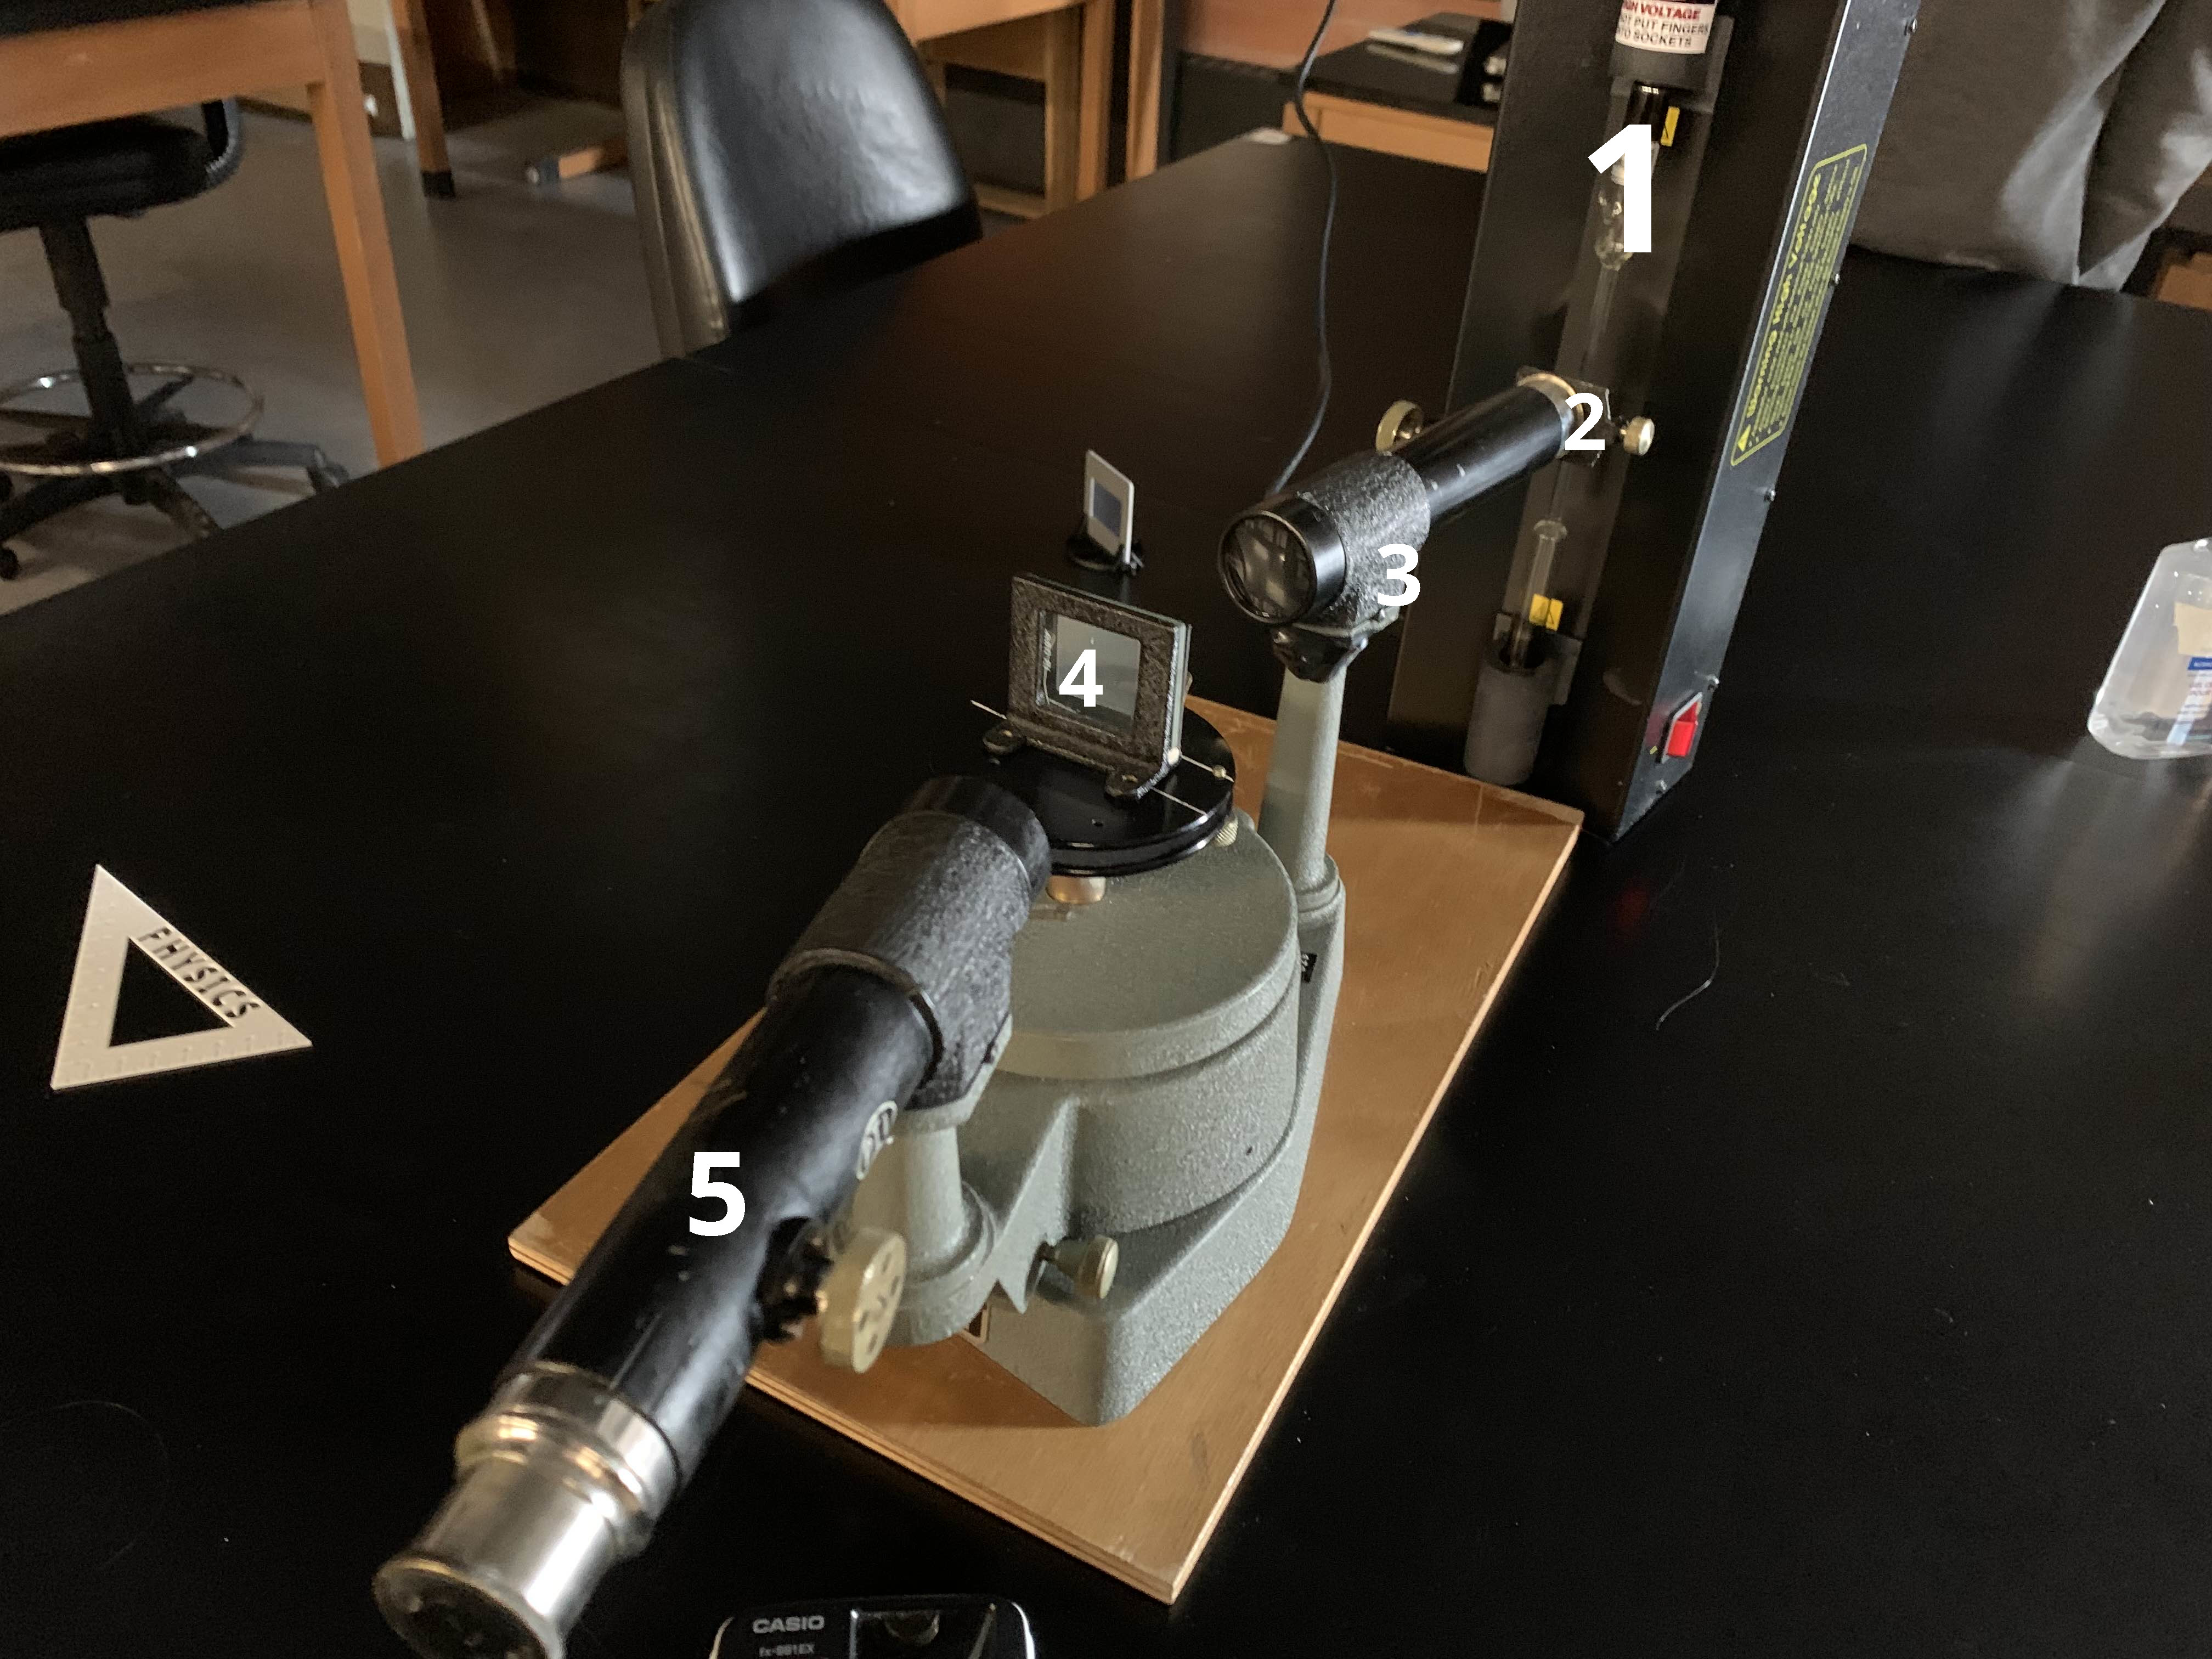
\includegraphics[scale=0.1]{Apparatus.jpg}
  \label{app}
\end{figure*}

\begin{figure*}[h]
  \centering%
  \caption{Illustrated first order ($m=\pm1$) diffractions through a $k=\qty{1.5d4}{lines\per inch}$, not to scale.}
  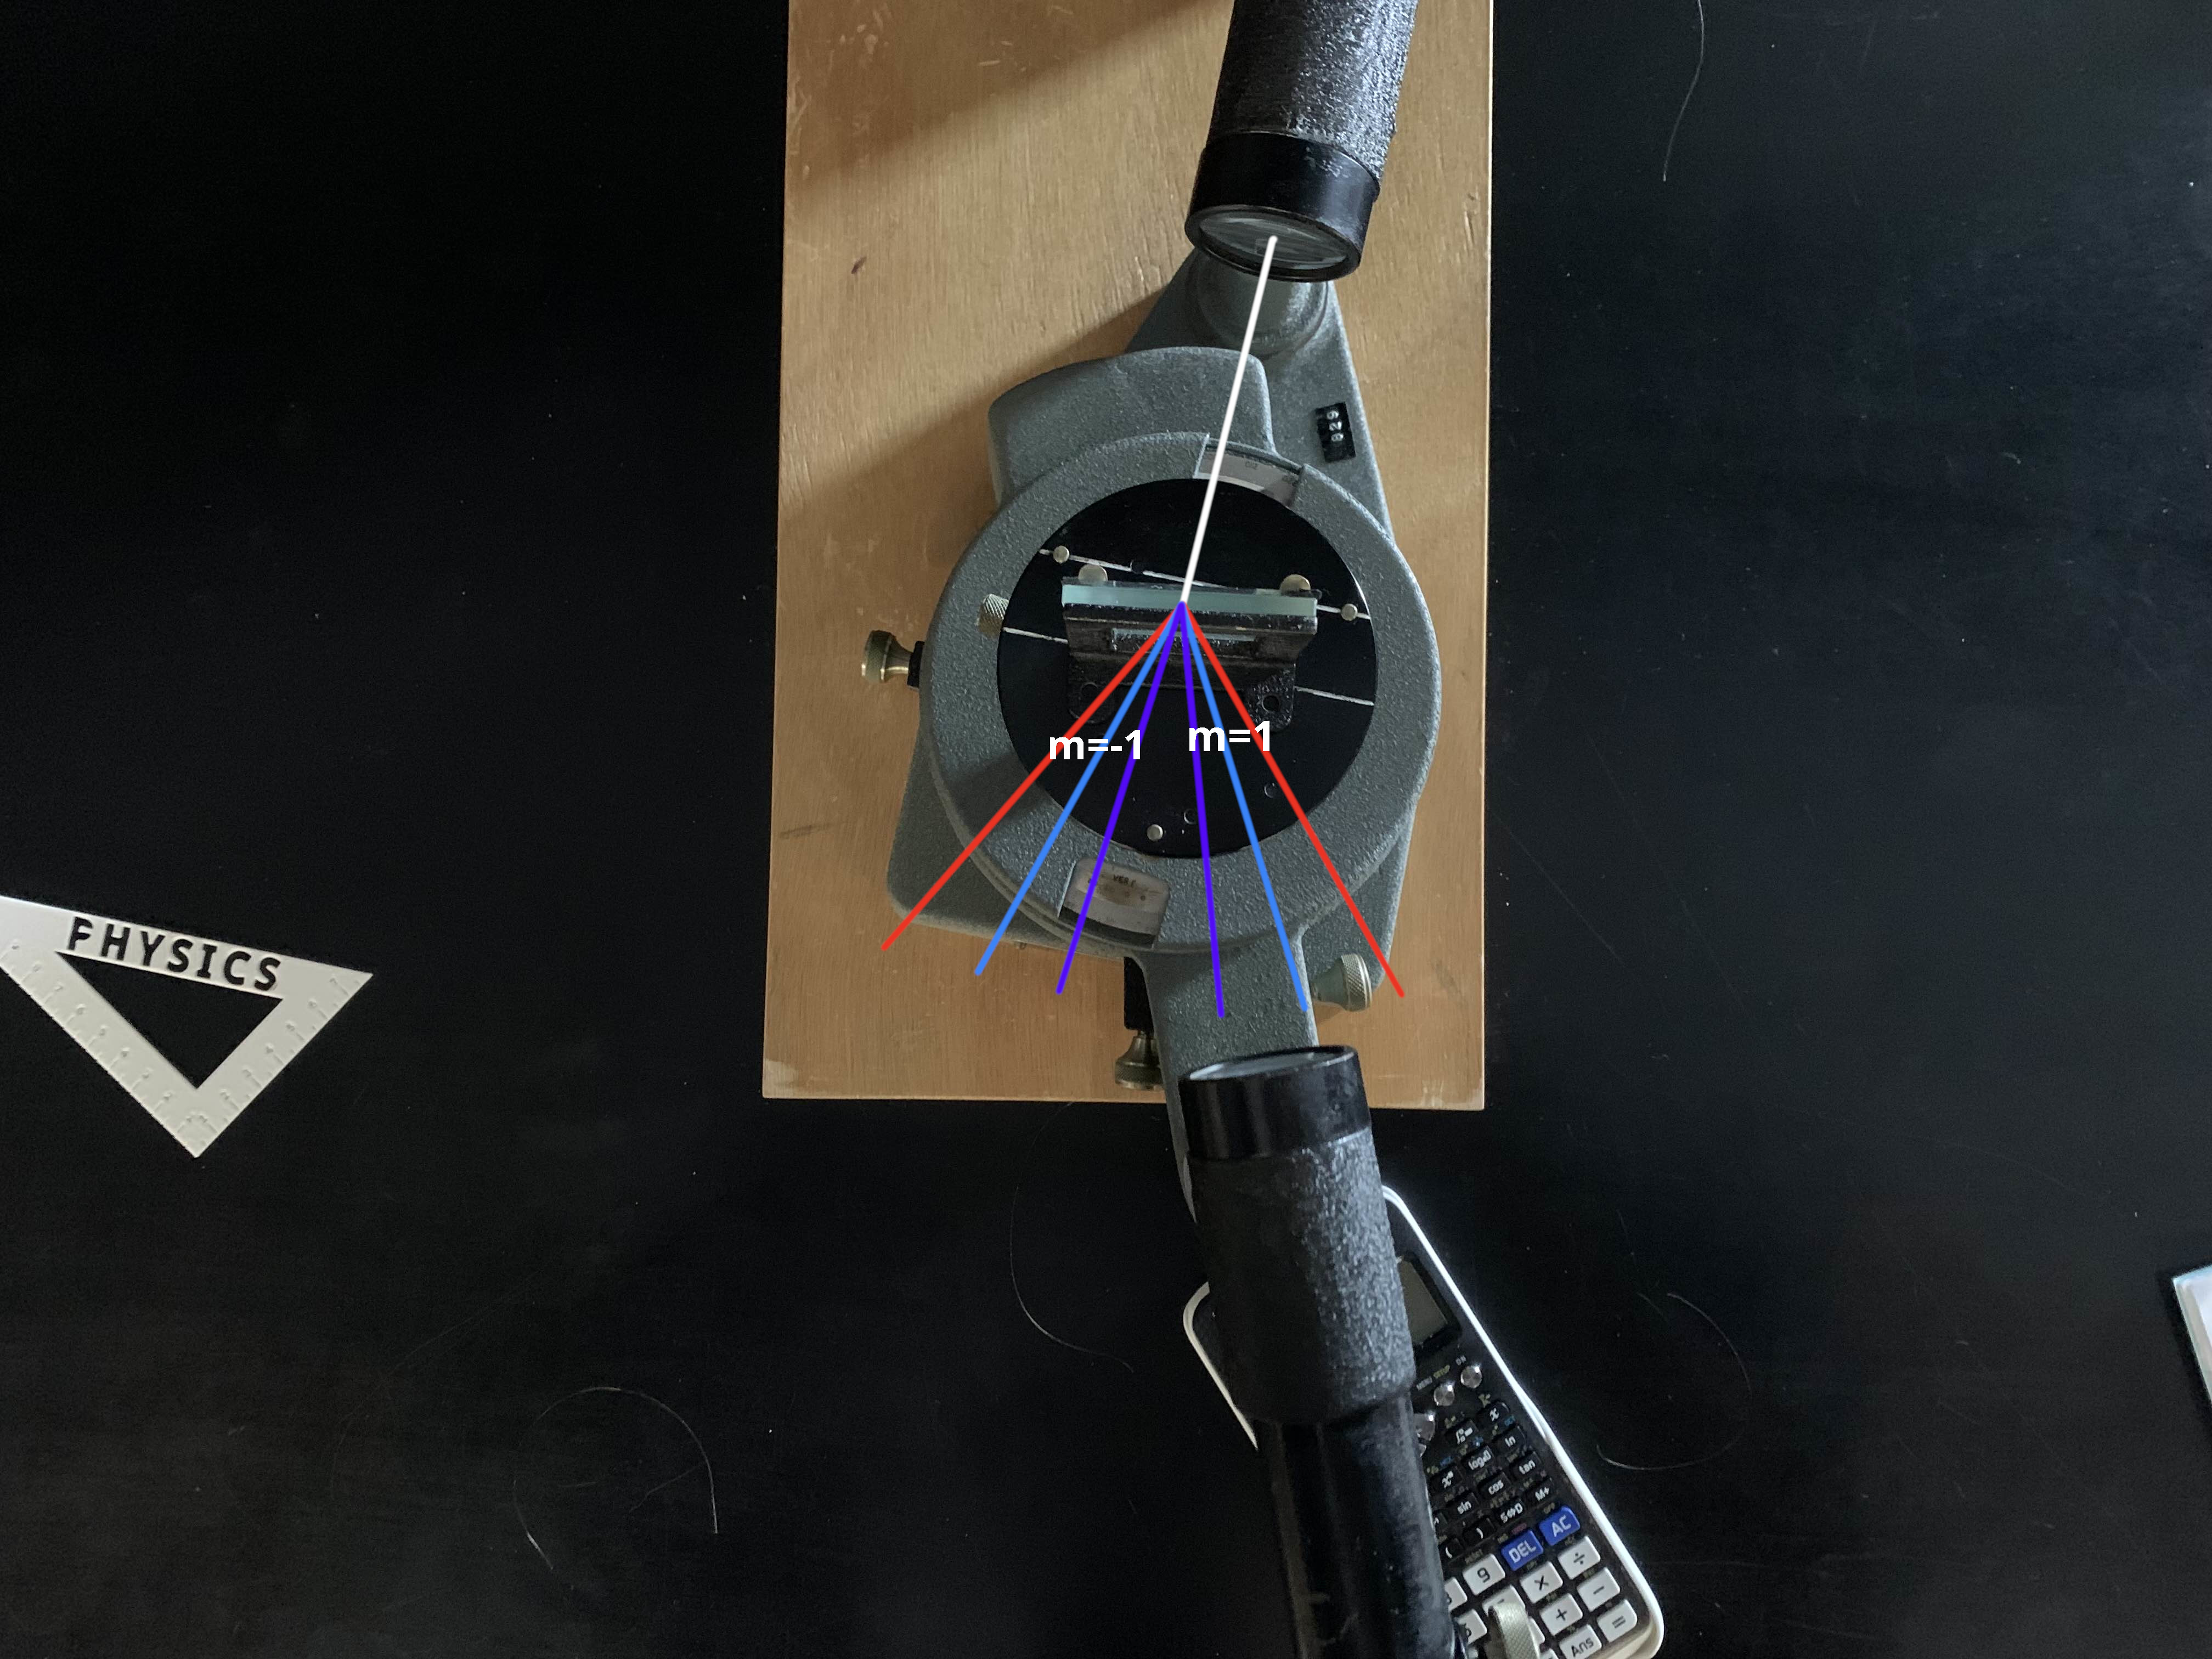
\includegraphics[scale=0.1]{Grating Above.jpg}
  \label{grat}
\end{figure*}

\begin{figure*}[h]
  \centering%
  \caption{Illustrated angles of minimum dispersion for a dense flint glass prism, not to scale.}
  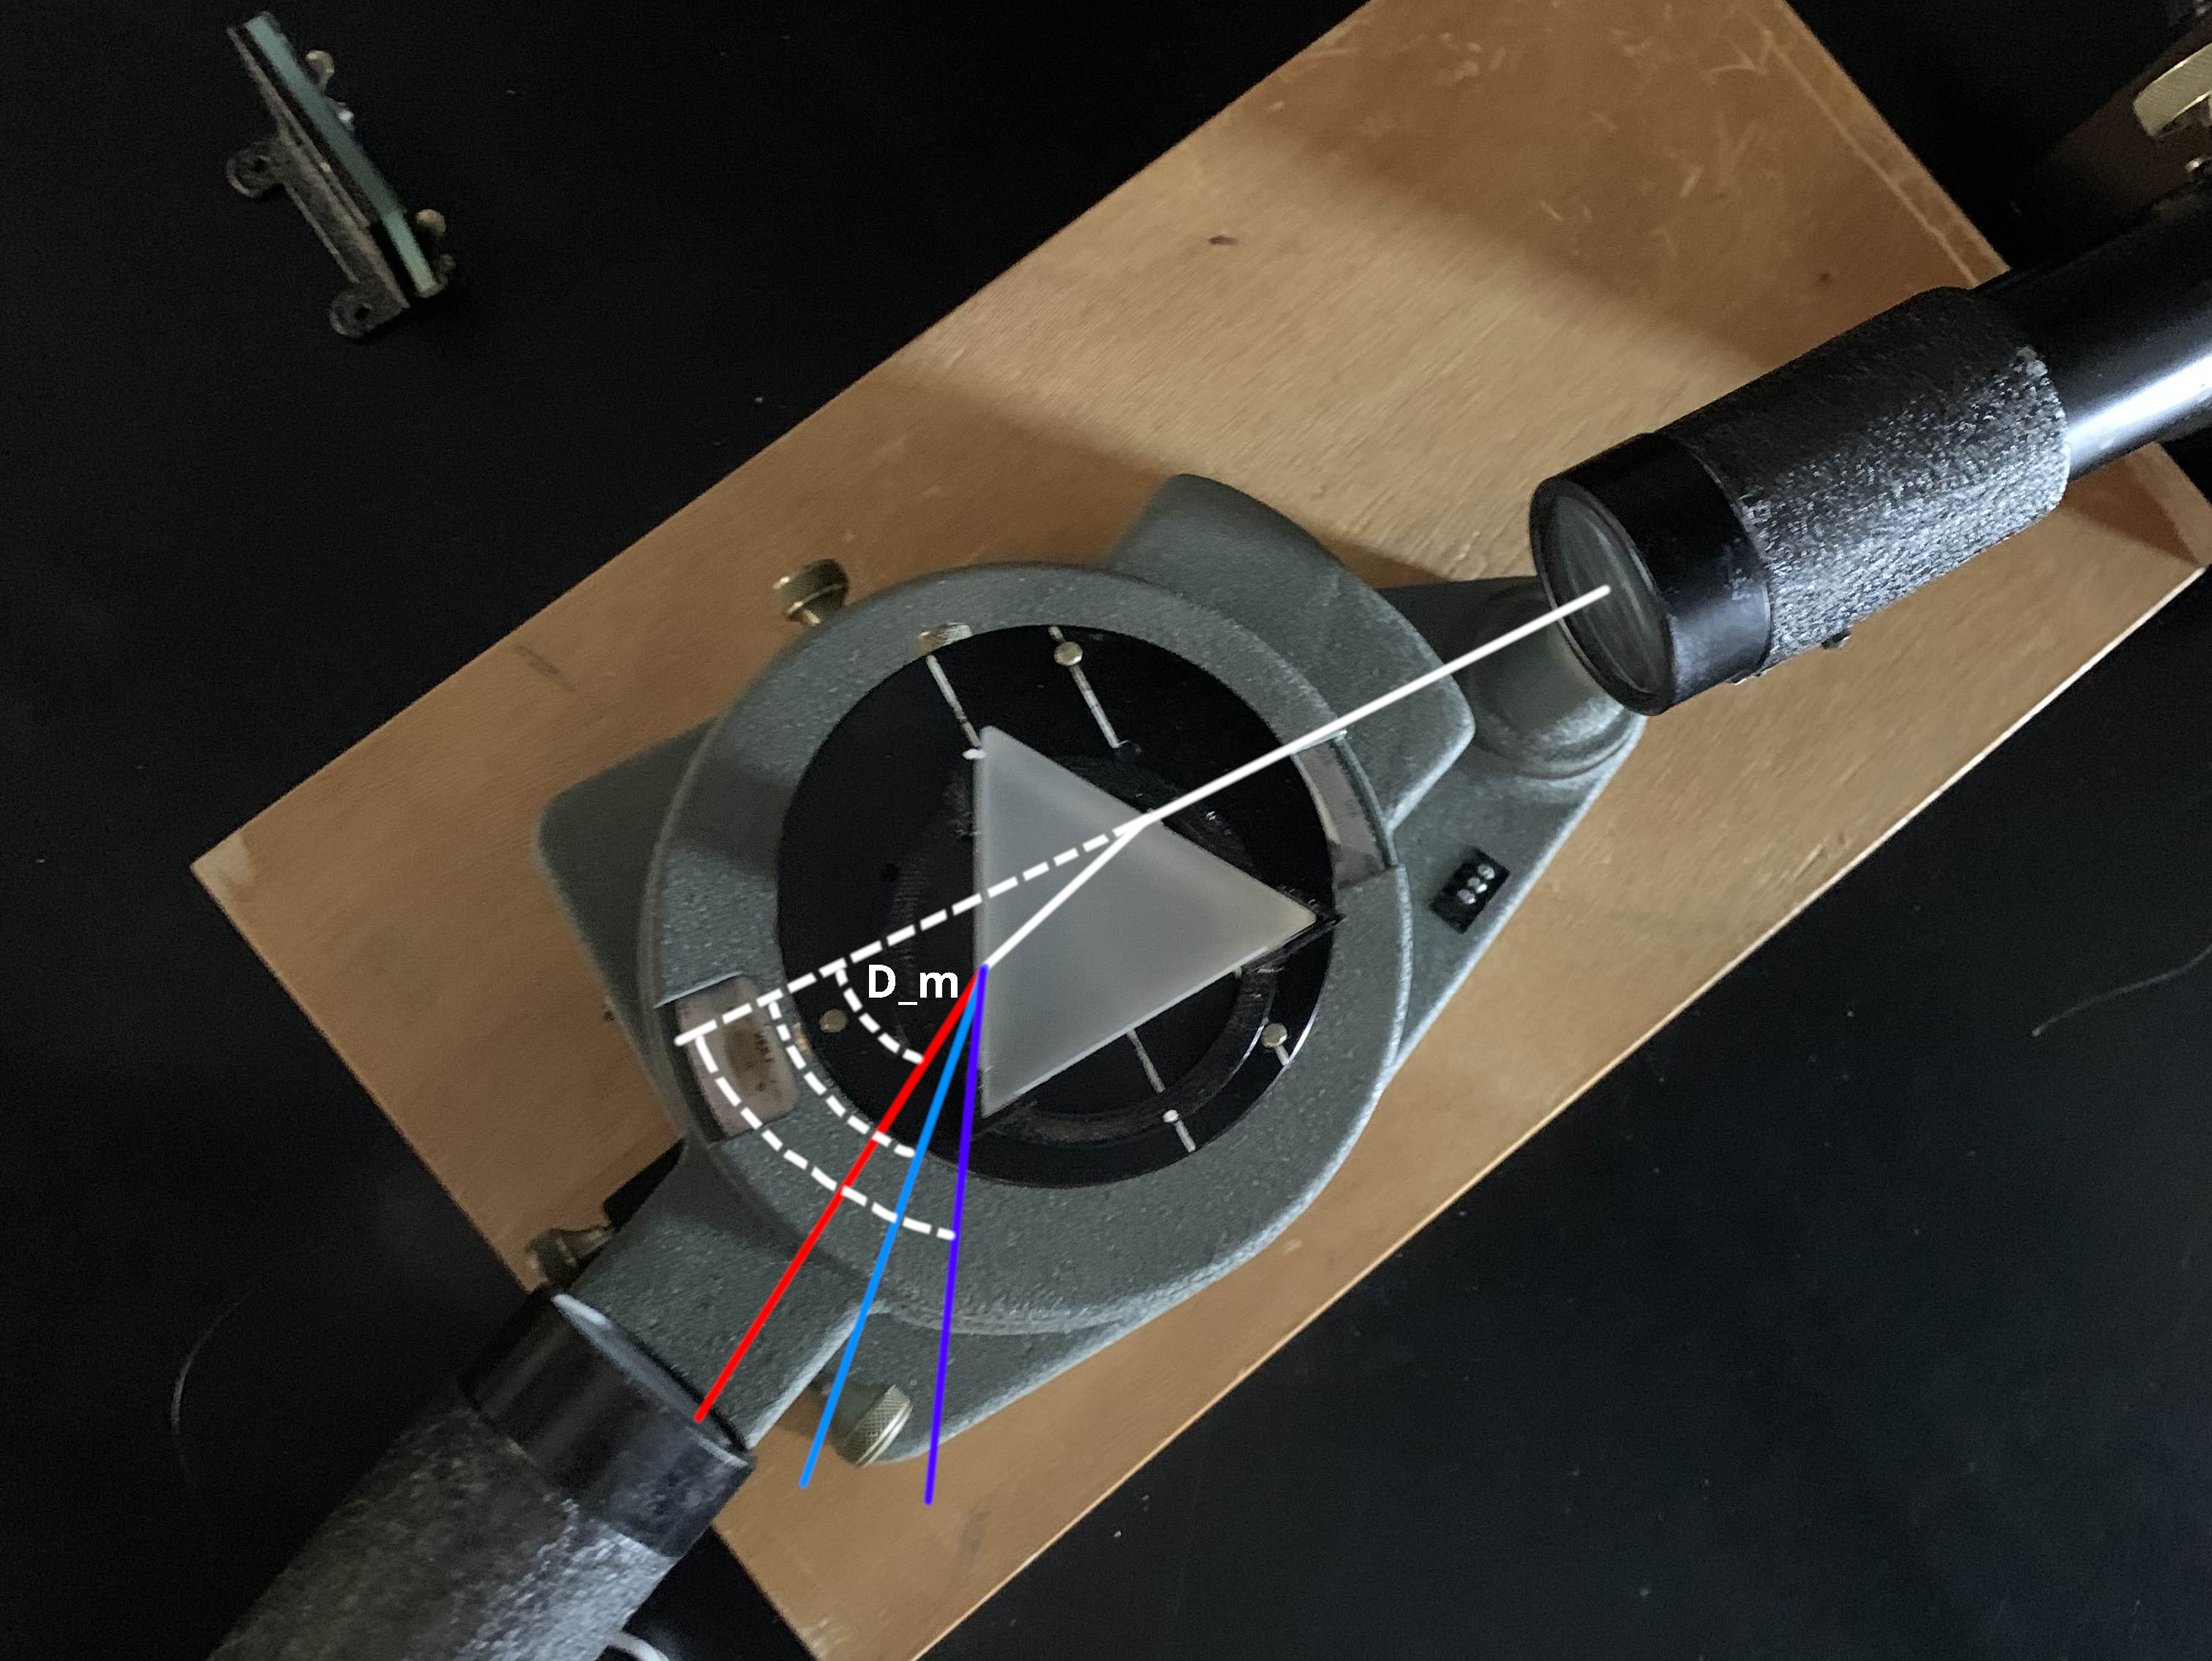
\includegraphics[scale=0.55]{Prism Above.jpg}
  \label{pris}
\end{figure*}
\end{document}